\begin{figure}[t]
\centering
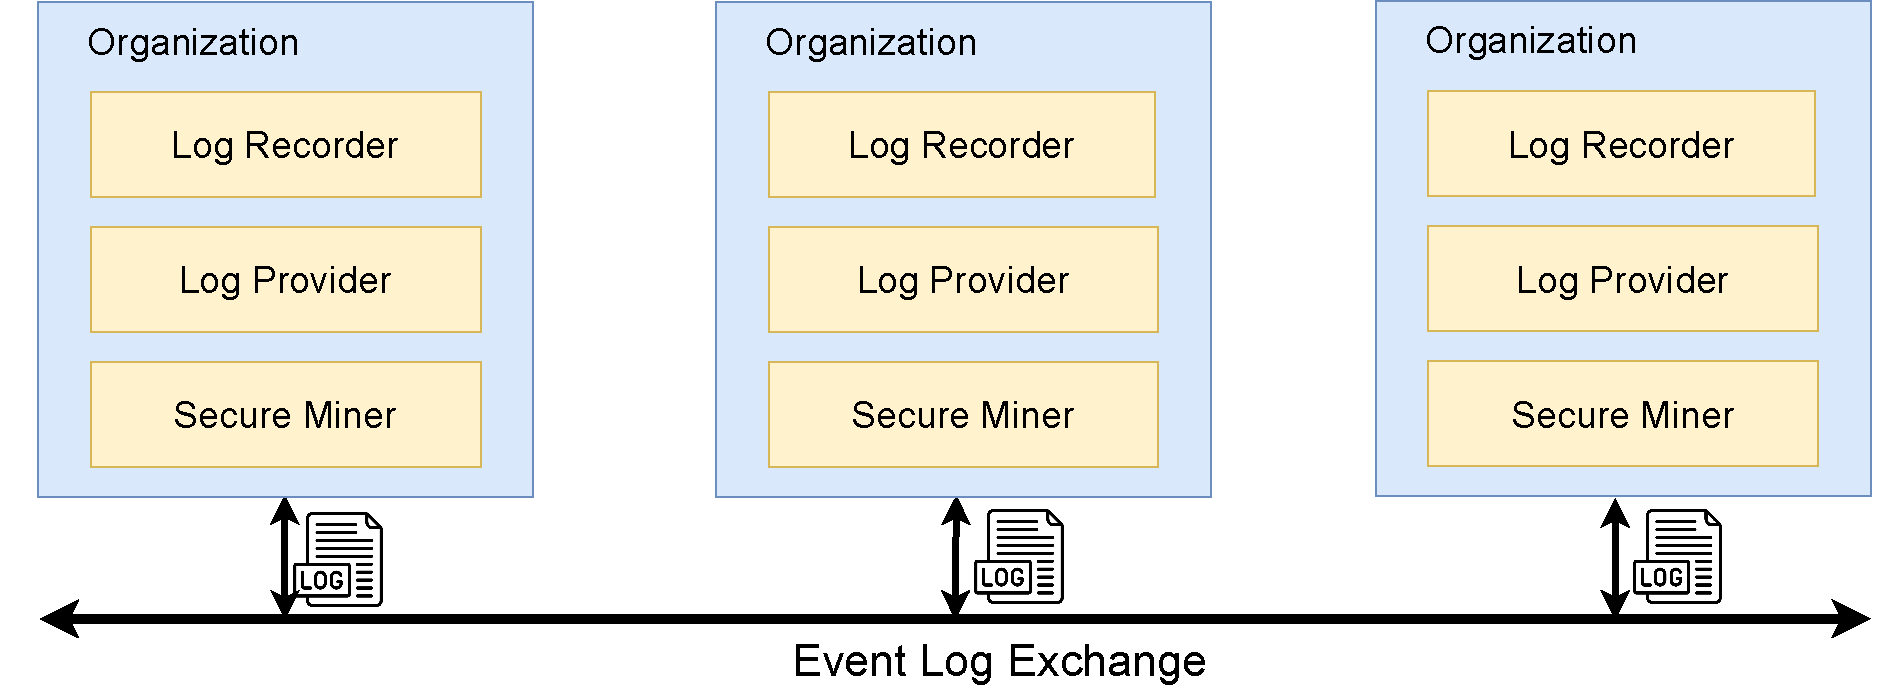
\includegraphics[width=11cm]{content/figures/architecture_diagram.pdf}
\caption{High-level architectural overview.}
\label{fig:architecture_diagram}
\end{figure}
In this section, we present the high-level architecture underlying our solution. We consider the main functionalities of each component, avoiding details on the employed technologies discussed in the next sections. Once we introduced the architecture, we focus on the \texttt{Secure Miner} component that represents the core of our contribution.
\todo{CDC: Do not use underscores in any circumstance, also NOT in labels or filenames. Look instead at Fig.~\ref{fig:architecture_diagram}, for example. Underscores create troubles in most of the cases as {\LaTeX} reserves that character for subscripts in math environments. We have gone through this too, so we should act as we know.}

\subsection{Architecture at large}
Our architecture involves networks of nodes controlled by different \texttt{Organization}s exchanging their event logs. \texttt{Organization}s in the same network collaborate to achieve a common objective and compose business processes whose event logs are scattered across multiple places. Therefore, each \texttt{Organization} produces event logs recording the operations executed to complete a business process. The hospital, the specialized clinic, and the pharmaceutical company mentioned in the running example provide an example of partner \texttt{Organization}s.
\todo[inline]{CDC: This is the last time we write something about the motivating scenario to exemplify our architecture until Section~\ref{sec:implementation:details}. Clearly, this is not OK. I have rejected papers for less.}

An \texttt{Organization} may assume one of the following two different roles or both: \textit{provider}, if it delivers local event logs to be collaboratively mined; a \textit{miner} whenever it applies process mining algorithms using local event logs in combination with ones generated by providers. In \cref{fig:architecture_diagram}, we propose a high-level schematization of our solution. Each \texttt{Organization} embeds four main components, which we describe next: the \texttt{Log Recorder}, the \texttt{Log Provider}, and the \texttt{Secure Miner}. The maintenance of event logs is the core task performed by \texttt{Log Recorder}. This component registers the events taking place in the \texttt{Organization}. The \texttt{Log Recorder} is queried by the local \texttt{Log Provider} for event logs to be fed into \texttt{Secure Miner}s. The \texttt{Log Provider} component delivers on-demand data to \texttt{Secure Miner}s. It controls access to local event logs by authenticating data requests generated by miners. \texttt{Log Provider}s reject demands from unauthorizated parties and only permit \texttt{Secure Miners} of partner \texttt{Organizations} to use the data. The \texttt{Secure Miner} shelters external event logs inside an \texttt{Organization}'s system by preserving data confidentiality and integrity. We provide an in-depth focus on this component as follows.
\todo{CDC: Figure widths should NEVER be absolute in terms of centimeters or so. They should always be a fraction of \texttt{textwidth} or \texttt{pageheight}. Otherwise, if we change a template (which is very likely, either because of extended versions of the paper or because sooner or later you might end up writing your PhD thesis), dimensions could all be screwed up. Look at Figs.~\ref{fig:architecture_diagram}~and~\ref{fig:trusted_miner} instead. We have gone through this too, so we should act as we know.}

\begin{figure}[t]
	\centering
	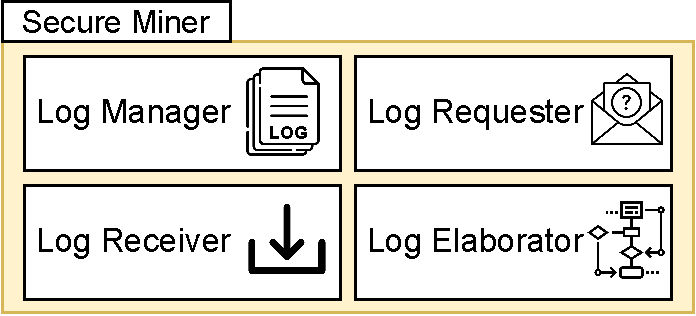
\includegraphics[width=0.6\linewidth]{content/figures/secure_miner.pdf}
	\caption{Subcomponents of the Secure Miner.}
	\label{fig:trusted_miner}
\end{figure}




\subsection{Secure Miner}
%The \texttt{Secure Miner} is a trusted application running inside the \texttt{Reserved Zone} that makes its source code and data tamper-proof. 
The primary objective of the \texttt{Secure Miner} is to allow \texttt{Organization}s to execute process mining algorithms using %local event logs alongside 
event logs retrieved from partner \texttt{Organization}s, ensuring fair data utilization to log providers. \texttt{Secure Miner}s leverage isolated execution contexts that guarantee tamper-proofing and data confidentiality. In \cref{fig:trusted_miner}, we show a schematization of a \texttt{Secure Miner} in which we distinguish four different subcomponents: the \texttt{Log Manager}, the \texttt{Log Requester}, the \texttt{Log Receiver}, and the \texttt{Log Elaborator}. Event logs belonging to partner \texttt{Organizaition}s are stored in the isolated execution context of the \texttt{Secure Miner}. We handle these data via the \texttt{Log Manager} that makes event log access not practicable from outside the \texttt{Secure Miner}'s execution context. Thus, the \texttt{Log Manager} prevents external parties from having direct access to event logs. These unauthorized entities include the owner of the miner \texttt{Organization} system. The \texttt{Log Requester} and the \texttt{Log Receiver} are the subcomponents that we employ during the event log exchange. \texttt{Log Requester}s initializes the exchange procedure and sends authenticable data requests to the \texttt{Data Provision} module of log providers. The \texttt{Log Receiver} collects event logs sent by \texttt{Log Providers} and entrusts them to the \texttt{Log Manager}. When collecting data, \texttt{Log Receiver}s prove their trustworthiness to \texttt{Log Provider}s by delivering evidence that certifies the \texttt{Secure Miner}'s execution context. The \texttt{Log Elaborator} is the core module of the \texttt{Secure Miner}. It collects the logic to securely execute process mining algorithms. 
When activated, the \texttt{Log Elaborator} accesses external event logs inside the \texttt{Secure Miner} and integrates them with the local event log of the \texttt{Organization}. We refer to this procedure as \textit{merging}. During the merging, the \texttt{Log Elaborator} enriches local traces with events belonging to logs from partner \texttt{Organization}s.



\begin{comment}
	\subsection{Workflow}
	% \label{sec:architecture:workflow}
	\subsubsection{Initialization}
	\subsubsection{Data Exchange}
	%The goal of the authentication procedure is to extract the public key representing the identity of the sending \texttt{Secure Miner}.
	%Remote Attestation and Log Segmentation are crucial procedures handled by the \texttt{Log Provider} during the provision process. Through Remote Attestation, \texttt{Log Provider}s verify that the \texttt{Secure Miner} that has generated the log request  is: (i) a known software object running inside a Reserved Zone; (ii) controlled by a partner \texttt{Organization} that has rights to access the event log. We named Log Segementation the process through which \texttt{Log Provider}s split the event log to be delivered in sub-log of smaller size.
	\subsubsection{Data Elaboration}
	
	
\end{comment}
